% This is the term paper for the CSCW class for which the tool Impact!
% was created and evaluated. This was done solely by Jordan Ell

\documentclass[conference]{IEEEtran}

\usepackage{graphicx}
\usepackage{amsmath}

\hyphenation{op-tical net-works semi-conduc-tor}

\begin{document}

%Paper title
\title{Creation of Developer Awareness Inside Changesets}

%Author block
\author{\IEEEauthorblockN{Jordan Ell}
\IEEEauthorblockA{University of Victoria,
Victoria, British Columbia \\ jell@uvic.ca}}

\maketitle

\begin{abstract}
Some abstract here.
\end{abstract}

\section{Introduction}

\section{Methodology}

The basis of the tool Impact is to create an information space which developers can see awareness information
based on the code they have written at the method level of source code. Impact will provide information to the
developer based on method ownership and those method's call hierarchies effected by changesets.  To preform
these actions, a two step approach will now be described. \\

\subsection{Extracting Technical Networks}
To extract the information needed for the Impact awareness tool, the source code repository must be queried to
extract information such as method ownership and method call hierarchies during a changeset. This information
will provide technical dependency edges between developers caused by changesets which can then be used as
awareness information and provided to the developers. \\

At each changeset, the method call graphs must be constructed. Method call graphs are a simple graph which uses
method declarations as nodes and method invocations as directed edges. To construct the call graphs, the source 
code repository (in this case Git) must be queried to obtain all source files of the project. Once all source files are
obtained, abstract syntax trees (AST) are then compiled for each file. The abstract syntax trees contain all information
in regards to the method call hierarchies of the project. From here, the call hierarchies can be constructed by simply
querying the ASTs in regards to method call structures. The method call graphs have now been constructed.\\

Once the method call graph has been constructed, the changeset can be used to identify the Impacted methods
of the changeset which will be used for developer awareness information. The Git repository now needs to be
queried in order to identify which methods have been changed by the changeset. This information can be 
extracted by using the "git diff" command. This command lists all information regarding files and lines
changed inside of a changeset. This information can then be put against the method call graphs as it is now 
known which lines of files, leading to which method, have been changed inside of the changeset. With each
changed method now found, a final query is made against the call graph to find those methods which invoke
the changed methods. These methods which invoke those changed will become the basis for the awareness
information to presented to developers. \\

Next, each invoking method inside of the call graph must be assigned weighted owners. The owners of a method are obtained
by using the Git repository. Git stores which developers have written which lines of code inside of a project, including
other information such as which changeset the line of code comes from and time and date. This information can be
retrieved by using the "git blame" command. To obtain weighted owners for each method a simple weight of number 
of lines written divided by total lines inside the method is given to each owner who is partially responsible for writing
each method. The weight method owners have now been obtained. \\

Between the method call graphs, identified changed and invoking methods of a changeset and their owners,
final developer network can now be constructed. This construction can be seen inside of Figure~\ref{fig:network}.
Here the method call graph between methods bar(), foo() and getX() has been constracuted with its owners
( Figure~\ref{fig:network} left hand side).
Inside of Carl's changeset, the function getX() has been modified. Since Impact is only interesting in developer
awareness and not method awareness, the network is simplified to involve only developers
( Figure~\ref{fig:network} right hand side). The awareness information is now ready to be presented to the
developers. \\

% Technical network figure
\begin{figure*}[tb!]
\centering
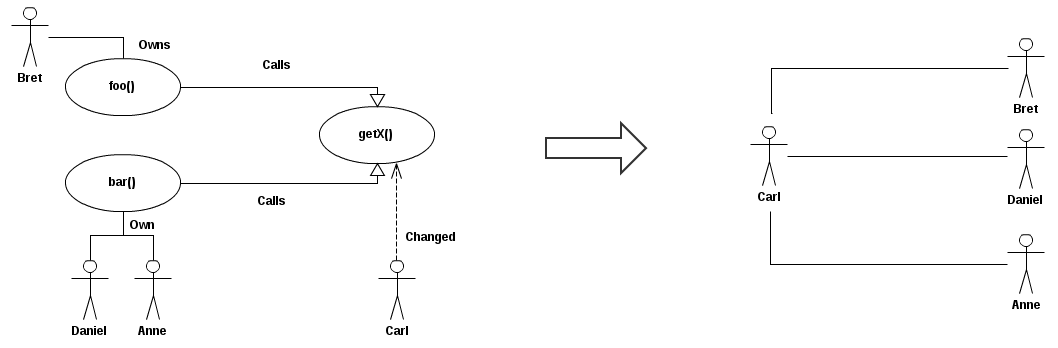
\includegraphics[width=0.9\textwidth]{images/TecNetwork}
\caption{A technical network with resulting developer network for a code change. Carl has changed method getX() which is being
called by Bret's method foo() as well as Daniel and Anne's method bar().\label{fig:network}}
\end{figure*}

\subsection{Providing Awareness Information}
For Impact to provide appropriate awareness information to the correct developer, three steps must be taken.
First the source code repository must be updated. Second the awareness information must be gathered from 
the repository. Lastly, the information must be stored in a database and presented to the developer in an 
appealing manner. \\

In order to update the code repository when new changesets are committed, a service hook must be used.
A service hook is a trigger stored on the project's central repository which sends information to an outside
server whenever activity with the central repository occurs (in this case a new changeset). A git hook is installed
on the project's central repository and hooked up to the Impact server being run. Once the Impact server 
receives the notification that a new changeset has been committed, Impact updates its local repository to
reflect this new changeset. From here the Impact tool proceeds to gather the awareness information needed
for the developers. \\

The awareness information is then gathered in the manner described in the previous subsection. Once the 
information has been gathered, it is stored inside of a local database on the Impact server for later use.\\

Now that the Impact server has the ability to gather and store information regarding the project's source code
repository, a front end must be used for developers to see the appropriate information. This front end
takes the form of a web application. Developers can visit the Impact server using a web browser in order to
see their awareness information. Developers are able to log into the Impact server using the same credentials 
as their source code repository and are then presented with RSS type feeds with awareness information.
The feeds can be used for tracking many different objects at the developers request, but the main purpose
is to display the awareness information gathered in the last subsection. This feed is called the Method Impact
feed and can be seen in Figure~\ref{fig:impact} as the left most feed. Here developers can see their methods
which have been impacted by other developer's changesets inside of the project. \\

The other types of feeds which are supported by Impact are Person and File feeds which can be seen as
the central and right most feeds respectively in Figure~\ref{fig:impact}.\\

%Impact figure
\begin{figure*}[tb!]
\centering
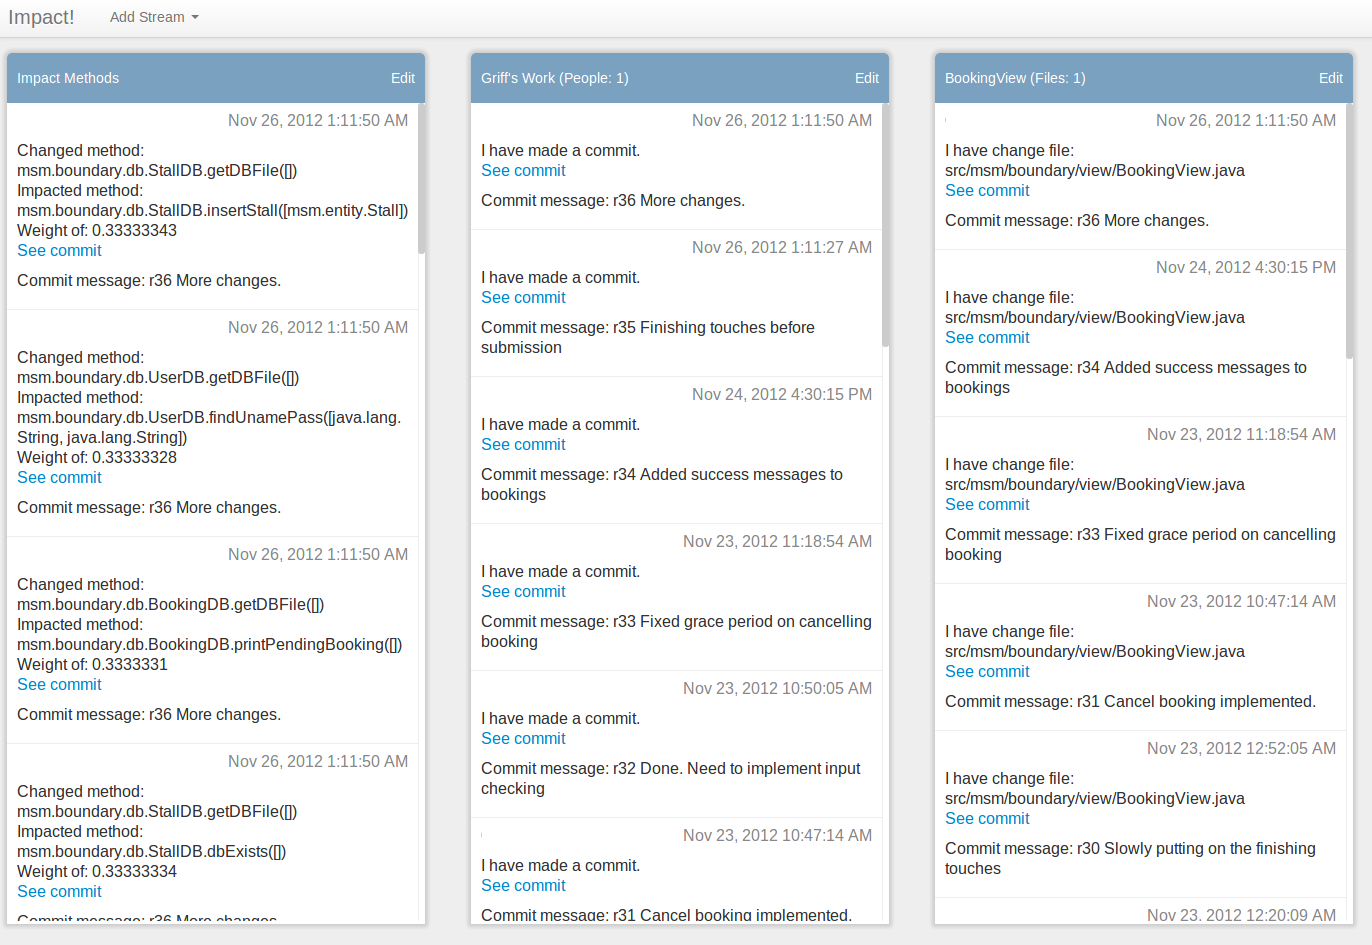
\includegraphics[width=0.9\textwidth]{images/ImpactDemo}
\caption{The tool Impact with developer names hidden.\label{fig:impact}}
\end{figure*}

\section{Evaluation}

\subsection{Participants}
In order to evaluate Impact, two case studies were used. The University of Victoria hosts an undergraduate
level class called Object Oriented Design (SENG 330) where students learn the practises of object oriented
programming languages and how design patterns can be used with these languages to achieve quality 
software applications. The course is taught with a hands on approach as student groups build a software
product over the course of the semester. Students go through all proper processes of building the product
such as requirements engineering, design, prototype/mock-ups, and final implementation. 
The final projects are presented at the end of semester. \\

A pitch for Impact was made in front of this class in order to request that teams use Impact as a tool during 
their development process. Two teams responded as willing participants for the use of Impact. Both teams 
had three members and were led by a core developer. \\

Team 1 was tasked with developing an arena bookings management system. The project was written in
Java and had a command line interface. The team was led by a 2nd year undergraduate student who was
also the core developer and backed up by two 3rd year undergraduates who also preformed minor
development. Team 1's lead developer Carl has had two years of development experience and is 
beginning to move into professional development.\\

Team 2 was tasked with developing a market management system. The project was written in Java
and used a Java Swing interface. The team was led by a 4th year undergraduate student who was
the sole developer of the project and also contained two 3rd year undergraduates. Team 2's lead
developer John has had 2 years of professional development experience and is involved in numerous
on going projects outside his professional career.\\

Each of the two teams was given an Impact server which was then used as a part of their development
process for the course project.

\subsection{Evaluation Strategy}
In order to evaluate the effectiveness of Impact in providing awareness information to the developers
on each of the two studied teams, semi-structured interviews were conducted with each of the team's
lead developers. A semi-structured interview was used as evaluating awareness applications is a
difficult task to approach with a formal structure. Questions were prepared ahead of time but, most
of the interviews ended up being spin off discussions from the original questions. Only the team's
lead developers were interviewed for multiple reasons. The first being these lead developers had the
most to benefit from the tool and had seen it in action most because of the larger amounts of
development done by these individuals. The second being these leads had the most external development
experience on their respective teams which allows them to approach the tool with knowledge of
other projects and its potential on them as well. The last being these developers produced most of
the source code for their respective projects which allowed them to use the tool more than the 
other members of their team.  \\

The interviews themselves focused on four areas of interest. The first being the developers background.
Establishing the interviewee as a competent developer with experience is crucial as the answers
provided about the tool need to be backed up by developer experience.  The second being determining
if bugs or problems arise in software these developers have worked on because of other developers
actions. These questions establish that Impact is attempting to solve a real world problem. This
is a crucial step in the interview which gives the tool legitimacy for future applications. The third
area of interest is understanding what types of actions other developers take which cause bugs
or unwanted processes in the developer's own code. These questions establish a domain of 
research. The hoping here is that the interviewees identify regions of source code which are
potentially harmful structures when changed by developers that can effect their own code. Impact
focuses on the method as the harmful structure. The final area of interest was a series of questions
which focused on conflict resolution. After the interviewee establish the existence of the problems
and provided a domain of knowledge, they were asked to explain how such conflicts were
discovered and resolved. \\

From the four areas listed above, it should be determinable whether or not Impact is a useful tool
without explicitly asking the developers. However, the developers were asked for their opinions 
on Impact as a tool for their team's development as well as its use in industry and what changes
they would make to the tool. \\

\section{Results}
This section will be broken up between in the responses of the two lead developers in regards to
the four areas of interview interest.

\subsection{Team 1 Lead Developer}
Team 1's lead developer, Carl, had a background of being a 2nd year computer science undergraduate
at the University of Victoria. He has been developing for just over 2 years but has yet to have real world
development experience although having had worked on several software projects outside of academia. \\

From the interview Carl had mentioned that he has faced numerous software bugs because of other changes
inside of the system. He has done bug fixing which he essentially related to fixing bugs caused by new
feature development which caused older code to fail. This establishes the fact that the problem Impact
is attempting to solve is a real world, the problem being other developers changesets effect other the
developer's own code in a negative way. In the third interview focus, Carl identified individual commits
as being a large contributor to producing bugs but more importantly he mentions that the source code
changes that occur as the result of merging Git branches can often cause his own code to have defects.
Carl also identified the modification of method parameter checking. Specifically, he mentioned that we
other developers as type of parameter value checking, it can cause bugs in his own code. An example is
that a developer changes a method to only accept a parameter of number greater than 0 compared to any
number. In the final area of the interview Carl spoke about the tools he used for conflict resolution. He
talked about his main tool being email for finding out what went wrong in a new changeset. He also
mentioned the use of GitHub which is an online resource for centralizing the git repository in order
to have a graphical view of other developer's changesets and manually searching for bug inducing 
code changes.\\ 

Carl's overall impression's of Impact is that it is a good starting point for this type of awareness tool.
He admitted to thinking that Impact could be a useful tool for large projects with multiple developers, however,
multiple changes to avoid information overload would need to be made. He suggested into only showing
high level impacts of his code to avoid being bombarded with too many messages about his code
being impacted. A final comment made by Carl was the suggestion of implementing public chat feeds
inside of the Impact tool to allow developers to communicate inside the tool rather than having to use
and external tool such as email for conflict resolution.\\

\subsection{Team 2 Lead Developer}
Team 2's lead developer, John, has a background of being a 4th year software engineer undergraduate
at the University of Victoria. He has been developing for 8 years and professionally developing for
4 of those years. John has been involved in 2 large scale software projects and has produced
many independent software projects.\\

From the interview John mentioned that he has faced real world scenarios where other developers
has introduced new features to a system that have resulted in him having to modify his own code
because of bugs that were introduced by the other developer. John estimated that approximately
once a week in his large software projects he would have to modify his own code because of what
other developers have change in the source code. John however also mentioned that in small scale project with 3
or less team members this was rarely a problem. John mentioned that some of the more harmful 
structures that could be changed by other developers which could Impact his are database schemas
and database interfaces. He also broadened the results to say any interface between modules
inside the source code can also cause major impact problems.  This of course would include the interfaces
to methods which can include results and inputs to methods. Lastly John mentioned the complexity
of time and space inside of method that he uses. If a method is changed to use more memory or
consume more time it can have a drastic effect on his own code or whether or not he chooses to
use those methods. For the last focus area of the interview in conflict resolution, John mentioned 
that he uses more advanced tools such as the "git blame" command mentioned earlier in this paper
to find out who wrote which lines of code for determining his social interactions.\\

John's final notes on the tool Impact were that he could see its usefulness in large scale software
development especially where not all developers are collocated. John mention that Impact is
heading in the right direction although he had some concerns about its information overload
right now. He suggested that not all changes to methods need to be reports. He thought that
interfaces to methods are a more important change then adding a new variable. He suggested
looking at what kinds of changes developers actually need to be aware of the most.\\

 

\section{Discussion}

\section{Threats To Validity}
The two threats to validity inside of the evaluation of Impact are the size of the evaluation
participants, and the participants expertise in the subject. The fact that only two teams had
used Impact during this evaluation and that only one member of each team was interviewed
leaves a large gap in the extrapolation of the answers given by the two team's lead 
developers. Two teams is not a large enough sample size to draw general conclusions
from the study. Two teams were only used for this study because of the large time constraints
of the study and the time constraints of willing participants. Secondly, the two developers
interviewed pose a large threat to validity as only one of them had real world development
experience and of that was under 5 years. Not having the background knowledge to make
judgement calls on what developers really want have hindered the results of this case study's 
results. \\

A finally but smaller threat to validity is that the projects being developed by the teams were
not real world applications. The projects being developed were part of a class project which
omits the severity of mistakes inside of the source code. Without the real world consequences
of bugs in software development, the teams may have been less concerned with the results
that the tool had to offer and thus have skewed the results of the study.\\

\section{Conclusion and Future Work}



\bibliographystyle{IEEEtran}
\bibliography{impact}

%End of paper
\end{document}